\documentclass[10pt]{article}
\usepackage[utf8]{inputenc}
 
\usepackage{geometry}
\usepackage{graphicx}

\geometry{portrait, margin=1.5in}
 
\begin{document}

\section{Exercise 2 - UML in practice}
\subsection{Exercise 2.1}
UML Aggregation applies to a "Consists of" relation.
Parts of the whole may be shared, which means that child classes can exist independent of the parent class.
If the parent is destroyed, the child can remain without the parent.

UML Composition applies to a "Contains" relation.
A part belongs to a whole. If the parent class does not exist, the child cannot exist separate of the parent. 
If the parent is destroyed, the child will also be destroyed.

Aggregation is used in the relations between the Game class and classes which assist the Game class.
A Game consists of multiple Units (players, aliens, barricades, explosions and bullets), Collisions and the alienController. These are a composition relation, because without these classes, it is not possible to play the game, thus making the Game class useless.

\subsection{Exercise  2.2}
Parameterized, generic classes use type parameters which enable the user to re-use code for a different object type. 

An example of a parametrized class used in the project is the java.util.ArrayList class.
It takes an input Type, and allows creation of a list, reusing the same code for every object type.

The project itself does not contain classes using Parameterized classes.

\subsection{Exercise  2.3}
The project contains one major hiararchy, treating the different game Units. 
Within the hierarchy there is a sub-hierarchy for bullets. There are two bullet types, one for aliens and one for the player.
The subclasses directly linked to Unit are "Polymorphism" relations, since the behavior of each unit is different.
The subclasses of Bullet are "Is-A" relations, since they have the same behavior as their superclass.

\begin{figure}[ht!]
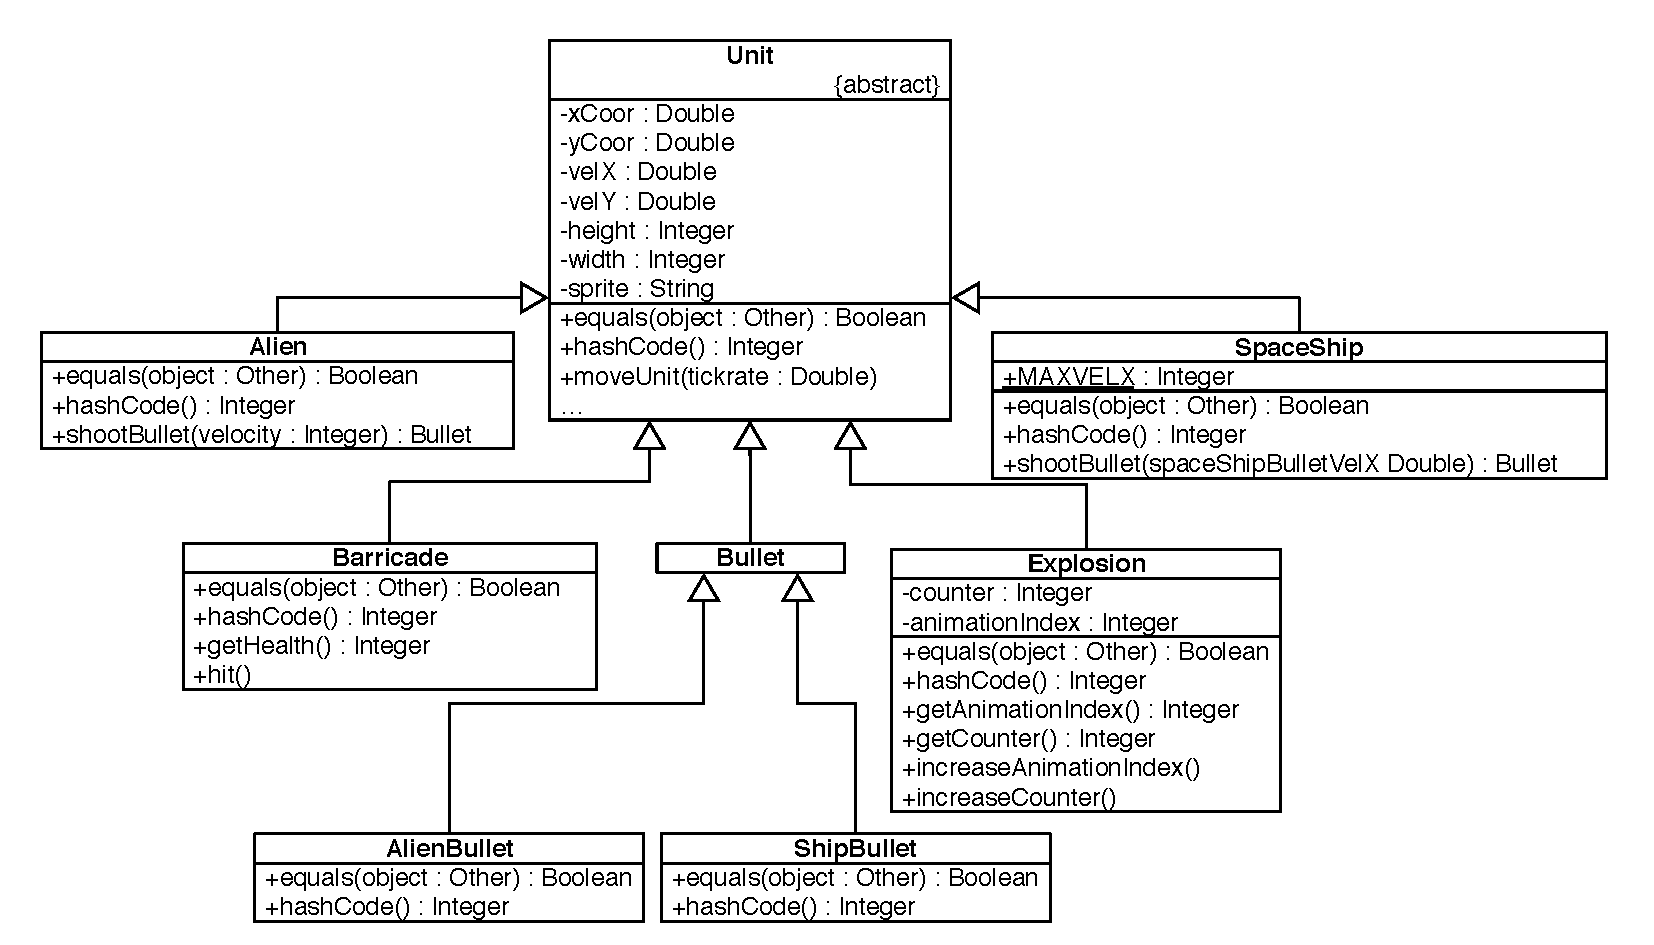
\includegraphics[width=1.1\textwidth]{SI-UMLhierarchies.pdf}
\end{figure}

\end{document}